% Options for packages loaded elsewhere
\PassOptionsToPackage{unicode}{hyperref}
\PassOptionsToPackage{hyphens}{url}
%
\documentclass[
]{book}
\usepackage{amsmath,amssymb}
\usepackage{lmodern}
\usepackage{ifxetex,ifluatex}
\ifnum 0\ifxetex 1\fi\ifluatex 1\fi=0 % if pdftex
  \usepackage[T1]{fontenc}
  \usepackage[utf8]{inputenc}
  \usepackage{textcomp} % provide euro and other symbols
\else % if luatex or xetex
  \usepackage{unicode-math}
  \defaultfontfeatures{Scale=MatchLowercase}
  \defaultfontfeatures[\rmfamily]{Ligatures=TeX,Scale=1}
\fi
% Use upquote if available, for straight quotes in verbatim environments
\IfFileExists{upquote.sty}{\usepackage{upquote}}{}
\IfFileExists{microtype.sty}{% use microtype if available
  \usepackage[]{microtype}
  \UseMicrotypeSet[protrusion]{basicmath} % disable protrusion for tt fonts
}{}
\makeatletter
\@ifundefined{KOMAClassName}{% if non-KOMA class
  \IfFileExists{parskip.sty}{%
    \usepackage{parskip}
  }{% else
    \setlength{\parindent}{0pt}
    \setlength{\parskip}{6pt plus 2pt minus 1pt}}
}{% if KOMA class
  \KOMAoptions{parskip=half}}
\makeatother
\usepackage{xcolor}
\IfFileExists{xurl.sty}{\usepackage{xurl}}{} % add URL line breaks if available
\IfFileExists{bookmark.sty}{\usepackage{bookmark}}{\usepackage{hyperref}}
\hypersetup{
  pdftitle={ハローワークデータからみる労働市場},
  pdfauthor={川田恵介},
  hidelinks,
  pdfcreator={LaTeX via pandoc}}
\urlstyle{same} % disable monospaced font for URLs
\usepackage{color}
\usepackage{fancyvrb}
\newcommand{\VerbBar}{|}
\newcommand{\VERB}{\Verb[commandchars=\\\{\}]}
\DefineVerbatimEnvironment{Highlighting}{Verbatim}{commandchars=\\\{\}}
% Add ',fontsize=\small' for more characters per line
\usepackage{framed}
\definecolor{shadecolor}{RGB}{248,248,248}
\newenvironment{Shaded}{\begin{snugshade}}{\end{snugshade}}
\newcommand{\AlertTok}[1]{\textcolor[rgb]{0.94,0.16,0.16}{#1}}
\newcommand{\AnnotationTok}[1]{\textcolor[rgb]{0.56,0.35,0.01}{\textbf{\textit{#1}}}}
\newcommand{\AttributeTok}[1]{\textcolor[rgb]{0.77,0.63,0.00}{#1}}
\newcommand{\BaseNTok}[1]{\textcolor[rgb]{0.00,0.00,0.81}{#1}}
\newcommand{\BuiltInTok}[1]{#1}
\newcommand{\CharTok}[1]{\textcolor[rgb]{0.31,0.60,0.02}{#1}}
\newcommand{\CommentTok}[1]{\textcolor[rgb]{0.56,0.35,0.01}{\textit{#1}}}
\newcommand{\CommentVarTok}[1]{\textcolor[rgb]{0.56,0.35,0.01}{\textbf{\textit{#1}}}}
\newcommand{\ConstantTok}[1]{\textcolor[rgb]{0.00,0.00,0.00}{#1}}
\newcommand{\ControlFlowTok}[1]{\textcolor[rgb]{0.13,0.29,0.53}{\textbf{#1}}}
\newcommand{\DataTypeTok}[1]{\textcolor[rgb]{0.13,0.29,0.53}{#1}}
\newcommand{\DecValTok}[1]{\textcolor[rgb]{0.00,0.00,0.81}{#1}}
\newcommand{\DocumentationTok}[1]{\textcolor[rgb]{0.56,0.35,0.01}{\textbf{\textit{#1}}}}
\newcommand{\ErrorTok}[1]{\textcolor[rgb]{0.64,0.00,0.00}{\textbf{#1}}}
\newcommand{\ExtensionTok}[1]{#1}
\newcommand{\FloatTok}[1]{\textcolor[rgb]{0.00,0.00,0.81}{#1}}
\newcommand{\FunctionTok}[1]{\textcolor[rgb]{0.00,0.00,0.00}{#1}}
\newcommand{\ImportTok}[1]{#1}
\newcommand{\InformationTok}[1]{\textcolor[rgb]{0.56,0.35,0.01}{\textbf{\textit{#1}}}}
\newcommand{\KeywordTok}[1]{\textcolor[rgb]{0.13,0.29,0.53}{\textbf{#1}}}
\newcommand{\NormalTok}[1]{#1}
\newcommand{\OperatorTok}[1]{\textcolor[rgb]{0.81,0.36,0.00}{\textbf{#1}}}
\newcommand{\OtherTok}[1]{\textcolor[rgb]{0.56,0.35,0.01}{#1}}
\newcommand{\PreprocessorTok}[1]{\textcolor[rgb]{0.56,0.35,0.01}{\textit{#1}}}
\newcommand{\RegionMarkerTok}[1]{#1}
\newcommand{\SpecialCharTok}[1]{\textcolor[rgb]{0.00,0.00,0.00}{#1}}
\newcommand{\SpecialStringTok}[1]{\textcolor[rgb]{0.31,0.60,0.02}{#1}}
\newcommand{\StringTok}[1]{\textcolor[rgb]{0.31,0.60,0.02}{#1}}
\newcommand{\VariableTok}[1]{\textcolor[rgb]{0.00,0.00,0.00}{#1}}
\newcommand{\VerbatimStringTok}[1]{\textcolor[rgb]{0.31,0.60,0.02}{#1}}
\newcommand{\WarningTok}[1]{\textcolor[rgb]{0.56,0.35,0.01}{\textbf{\textit{#1}}}}
\usepackage{longtable,booktabs,array}
\usepackage{calc} % for calculating minipage widths
% Correct order of tables after \paragraph or \subparagraph
\usepackage{etoolbox}
\makeatletter
\patchcmd\longtable{\par}{\if@noskipsec\mbox{}\fi\par}{}{}
\makeatother
% Allow footnotes in longtable head/foot
\IfFileExists{footnotehyper.sty}{\usepackage{footnotehyper}}{\usepackage{footnote}}
\makesavenoteenv{longtable}
\usepackage{graphicx}
\makeatletter
\def\maxwidth{\ifdim\Gin@nat@width>\linewidth\linewidth\else\Gin@nat@width\fi}
\def\maxheight{\ifdim\Gin@nat@height>\textheight\textheight\else\Gin@nat@height\fi}
\makeatother
% Scale images if necessary, so that they will not overflow the page
% margins by default, and it is still possible to overwrite the defaults
% using explicit options in \includegraphics[width, height, ...]{}
\setkeys{Gin}{width=\maxwidth,height=\maxheight,keepaspectratio}
% Set default figure placement to htbp
\makeatletter
\def\fps@figure{htbp}
\makeatother
\setlength{\emergencystretch}{3em} % prevent overfull lines
\providecommand{\tightlist}{%
  \setlength{\itemsep}{0pt}\setlength{\parskip}{0pt}}
\setcounter{secnumdepth}{5}
\usepackage{booktabs}
\ifluatex
  \usepackage{selnolig}  % disable illegal ligatures
\fi
\usepackage[]{natbib}
\bibliographystyle{apalike}

\title{ハローワークデータからみる労働市場}
\author{川田恵介}
\date{2021-07-31}

\begin{document}
\maketitle

{
\setcounter{tocdepth}{1}
\tableofcontents
}
\begin{Shaded}
\begin{Highlighting}[]
\NormalTok{pacman}\SpecialCharTok{::}\FunctionTok{p\_load}\NormalTok{(}\StringTok{"tidyverse"}\NormalTok{,}
               \StringTok{"readxl"}\NormalTok{,}
               \StringTok{"lubridate"}\NormalTok{,}
               \StringTok{"knitr"}\NormalTok{)}
\end{Highlighting}
\end{Shaded}

\hypertarget{ux8981ux7d04}{%
\chapter{要約}\label{ux8981ux7d04}}

公的職業紹介業務(ハローワーク)を通じて収集された業務データ(職業安定業務統計)を用いて、日本の求人・求職の状況を概観する。

\hypertarget{ux8a18ux8ff0ux7d71ux8a08ux91cf}{%
\chapter{記述統計量}\label{ux8a18ux8ff0ux7d71ux8a08ux91cf}}

\begin{itemize}
\tightlist
\item
  1963年から2020年までの月次データを用いて、厚生変化を記述する
\end{itemize}

\hypertarget{ux65b9ux6cd5}{%
\section{方法}\label{ux65b9ux6cd5}}

\begin{itemize}
\item
  期別に集計
\item
  季節性を除去するために、前年同月対数差を報告
\end{itemize}

\[\log(Y_{year,quaterly})-\log(Y_{year-1,quaterly})\]

\hypertarget{rux30b3ux30fcux30c9}{%
\section{Rコード}\label{rux30b3ux30fcux30c9}}

\begin{Shaded}
\begin{Highlighting}[]
\NormalTok{col.label }\OtherTok{\textless{}{-}} 
   \FunctionTok{c}\NormalTok{(}\StringTok{"year"}\NormalTok{,}
     \StringTok{"1"}\NormalTok{,}
     \StringTok{"2"}\NormalTok{,}
     \StringTok{"3"}\NormalTok{,}
     \StringTok{"4"}\NormalTok{,}
     \StringTok{"5"}\NormalTok{,}
     \StringTok{"6"}\NormalTok{,}
     \StringTok{"7"}\NormalTok{,}
     \StringTok{"8"}\NormalTok{,}
     \StringTok{"9"}\NormalTok{,}
     \StringTok{"10"}\NormalTok{,}
     \StringTok{"11"}\NormalTok{,}
     \StringTok{"12"}\NormalTok{,}
     \StringTok{"type"}\NormalTok{,}
     \StringTok{"group"}\NormalTok{)}

\NormalTok{select.raw }\OtherTok{\textless{}{-}} \DecValTok{14}\SpecialCharTok{:}\DecValTok{63}

\NormalTok{select.column }\OtherTok{\textless{}{-}} \FunctionTok{c}\NormalTok{(}\DecValTok{1}\NormalTok{,}\DecValTok{3}\SpecialCharTok{:}\DecValTok{14}\NormalTok{)}

\NormalTok{raw.vacancy.full }\OtherTok{\textless{}{-}}
  \FunctionTok{read\_excel}\NormalTok{(}\StringTok{"data/第6表.xlsx"}\NormalTok{,}
             \AttributeTok{sheet =} \StringTok{"第6表ー2(パート除く)"}\NormalTok{) }\SpecialCharTok{\%\textgreater{}\%}
\NormalTok{  .[select.raw,select.column] }\SpecialCharTok{|}\ErrorTok{\textgreater{}} 
  \FunctionTok{mutate}\NormalTok{(}\AttributeTok{type =} \StringTok{"求人"}\NormalTok{,}
         \AttributeTok{group =} \StringTok{"フルタイム"}\NormalTok{)}

\FunctionTok{colnames}\NormalTok{(raw.vacancy.full) }\OtherTok{\textless{}{-}}\NormalTok{ col.label}

\NormalTok{raw.seeker.full }\OtherTok{\textless{}{-}}
  \FunctionTok{read\_excel}\NormalTok{(}\StringTok{"data/第7表.xlsx"}\NormalTok{,}
             \AttributeTok{sheet =} \StringTok{"第7表ー2(パート除く)"}\NormalTok{) }\SpecialCharTok{\%\textgreater{}\%}
\NormalTok{  .[select.raw,select.column] }\SpecialCharTok{|}\ErrorTok{\textgreater{}} 
  \FunctionTok{mutate}\NormalTok{(}\AttributeTok{type =} \StringTok{"求職"}\NormalTok{,}
         \AttributeTok{group =} \StringTok{"フルタイム"}\NormalTok{)}

\FunctionTok{colnames}\NormalTok{(raw.seeker.full) }\OtherTok{\textless{}{-}}\NormalTok{ col.label}

\NormalTok{raw.hir.full }\OtherTok{\textless{}{-}}
  \FunctionTok{read\_excel}\NormalTok{(}\StringTok{"data/第8表.xlsx"}\NormalTok{,}
             \AttributeTok{sheet =} \StringTok{"第8表ー2(パート除く)"}\NormalTok{) }\SpecialCharTok{\%\textgreater{}\%}
\NormalTok{  .[select.raw,select.column] }\SpecialCharTok{|}\ErrorTok{\textgreater{}} 
  \FunctionTok{mutate}\NormalTok{(}\AttributeTok{type =} \StringTok{"新規就職"}\NormalTok{,}
         \AttributeTok{group =} \StringTok{"フルタイム"}\NormalTok{)}

\FunctionTok{colnames}\NormalTok{(raw.hir.full) }\OtherTok{\textless{}{-}}\NormalTok{ col.label}


\NormalTok{raw.vacancy.part }\OtherTok{\textless{}{-}}
  \FunctionTok{read\_excel}\NormalTok{(}\StringTok{"data/第6表.xlsx"}\NormalTok{,}
             \AttributeTok{sheet =} \StringTok{"第6表ー3(パート)"}\NormalTok{) }\SpecialCharTok{\%\textgreater{}\%}
\NormalTok{  .[select.raw,select.column] }\SpecialCharTok{|}\ErrorTok{\textgreater{}} 
  \FunctionTok{mutate}\NormalTok{(}\AttributeTok{type =} \StringTok{"求人"}\NormalTok{,}
         \AttributeTok{group =} \StringTok{"パートタイム"}\NormalTok{)}

\FunctionTok{colnames}\NormalTok{(raw.vacancy.part) }\OtherTok{\textless{}{-}}\NormalTok{ col.label}

\NormalTok{raw.seeker.part }\OtherTok{\textless{}{-}}
  \FunctionTok{read\_excel}\NormalTok{(}\StringTok{"data/第7表.xlsx"}\NormalTok{,}
             \AttributeTok{sheet =} \StringTok{"第7表ー3(パート)"}\NormalTok{)  }\SpecialCharTok{\%\textgreater{}\%}
\NormalTok{  .[select.raw,select.column] }\SpecialCharTok{|}\ErrorTok{\textgreater{}} 
  \FunctionTok{mutate}\NormalTok{(}\AttributeTok{type =} \StringTok{"求職"}\NormalTok{,}
         \AttributeTok{group =} \StringTok{"パートタイム"}\NormalTok{)}

\FunctionTok{colnames}\NormalTok{(raw.seeker.part) }\OtherTok{\textless{}{-}}\NormalTok{ col.label}

\NormalTok{raw.hir.part }\OtherTok{\textless{}{-}}
  \FunctionTok{read\_excel}\NormalTok{(}\StringTok{"data/第8表.xlsx"}\NormalTok{,}
             \AttributeTok{sheet =} \StringTok{"第8表ー3(パート)"}\NormalTok{) }\SpecialCharTok{\%\textgreater{}\%}
\NormalTok{  .[select.raw,select.column] }\SpecialCharTok{|}\ErrorTok{\textgreater{}} 
  \FunctionTok{mutate}\NormalTok{(}\AttributeTok{type =} \StringTok{"新規就職"}\NormalTok{,}
         \AttributeTok{group =} \StringTok{"パートタイム"}\NormalTok{)}

\FunctionTok{colnames}\NormalTok{(raw.hir.part) }\OtherTok{\textless{}{-}}\NormalTok{ col.label}

\NormalTok{df }\OtherTok{\textless{}{-}}
  \FunctionTok{rbind}\NormalTok{(raw.hir.full,}
\NormalTok{        raw.hir.part,}
\NormalTok{        raw.vacancy.full,}
\NormalTok{        raw.vacancy.part,}
\NormalTok{        raw.seeker.full,}
\NormalTok{        raw.seeker.part}
\NormalTok{        ) }\SpecialCharTok{|}\ErrorTok{\textgreater{}} 
  \FunctionTok{pivot\_longer}\NormalTok{(}\AttributeTok{cols =} \DecValTok{2}\SpecialCharTok{:}\DecValTok{13}\NormalTok{,}
               \AttributeTok{names\_to =} \StringTok{"month"}\NormalTok{,}
               \AttributeTok{values\_to =} \StringTok{"n"}\NormalTok{) }\SpecialCharTok{|}\ErrorTok{\textgreater{}} 
  \FunctionTok{mutate}\NormalTok{(}\AttributeTok{n =}\NormalTok{ n }\SpecialCharTok{|}\ErrorTok{\textgreater{}} \FunctionTok{as.numeric}\NormalTok{(),}
         \AttributeTok{year =}\NormalTok{ year }\SpecialCharTok{|}\ErrorTok{\textgreater{}} \FunctionTok{str\_sub}\NormalTok{(}\DecValTok{1}\NormalTok{,}\DecValTok{4}\NormalTok{) }\SpecialCharTok{|}\ErrorTok{\textgreater{}} \FunctionTok{as.numeric}\NormalTok{(),}
         \AttributeTok{month =}\NormalTok{ month }\SpecialCharTok{|}\ErrorTok{\textgreater{}} \FunctionTok{as.numeric}\NormalTok{(),}
         \AttributeTok{quaterly =}\NormalTok{ month }\SpecialCharTok{|}\ErrorTok{\textgreater{}} \FunctionTok{cut}\NormalTok{(}\FunctionTok{c}\NormalTok{(}\DecValTok{0}\NormalTok{,}\DecValTok{3}\NormalTok{,}\DecValTok{6}\NormalTok{,}\DecValTok{9}\NormalTok{,}\DecValTok{12}\NormalTok{), }\AttributeTok{labels =} \FunctionTok{c}\NormalTok{(}\DecValTok{1}\NormalTok{,}\DecValTok{2}\NormalTok{,}\DecValTok{3}\NormalTok{,}\DecValTok{4}\NormalTok{)),}
         \AttributeTok{date =} \FunctionTok{yq}\NormalTok{(}\FunctionTok{str\_c}\NormalTok{(year,quaterly,}\AttributeTok{sep =} \StringTok{":Q"}\NormalTok{))}
\NormalTok{         ) }\SpecialCharTok{|}\ErrorTok{\textgreater{}} 
  \FunctionTok{group\_by}\NormalTok{(date,type) }\SpecialCharTok{|}\ErrorTok{\textgreater{}} 
  \FunctionTok{mutate}\NormalTok{(}\AttributeTok{n =}\NormalTok{ n }\SpecialCharTok{|}\ErrorTok{\textgreater{}} \FunctionTok{sum}\NormalTok{()) }\SpecialCharTok{|}\ErrorTok{\textgreater{}} 
  \FunctionTok{ungroup}\NormalTok{() }\SpecialCharTok{|}\ErrorTok{\textgreater{}} 
  \FunctionTok{distinct}\NormalTok{(year,quaterly,date,type,n) }\SpecialCharTok{|}\ErrorTok{\textgreater{}} 
  \FunctionTok{spread}\NormalTok{(}\AttributeTok{key =}\NormalTok{ type, }\AttributeTok{value =}\NormalTok{ n) }\SpecialCharTok{|}\ErrorTok{\textgreater{}} 
  \FunctionTok{group\_by}\NormalTok{(quaterly) }\SpecialCharTok{|}\ErrorTok{\textgreater{}} 
  \FunctionTok{mutate}\NormalTok{(求人 }\OtherTok{=} \FunctionTok{log}\NormalTok{(求人) }\SpecialCharTok{{-}} \FunctionTok{log}\NormalTok{(}\FunctionTok{lag}\NormalTok{(求人)),}
\NormalTok{           求職 }\OtherTok{=} \FunctionTok{log}\NormalTok{(求職) }\SpecialCharTok{{-}} \FunctionTok{log}\NormalTok{(}\FunctionTok{lag}\NormalTok{(求職)),}
\NormalTok{           新規就職 }\OtherTok{=} \FunctionTok{log}\NormalTok{(新規就職) }\SpecialCharTok{{-}} \FunctionTok{log}\NormalTok{(}\FunctionTok{lag}\NormalTok{(新規就職))}
\NormalTok{           ) }\SpecialCharTok{|}\ErrorTok{\textgreater{}} 
  \FunctionTok{ungroup}\NormalTok{() }\SpecialCharTok{|}\ErrorTok{\textgreater{}} 
  \FunctionTok{pivot\_longer}\NormalTok{(}\AttributeTok{cols =} \FunctionTok{c}\NormalTok{(}\DecValTok{4}\SpecialCharTok{:}\DecValTok{6}\NormalTok{),}
               \AttributeTok{names\_to =} \StringTok{"type"}\NormalTok{,}
               \AttributeTok{values\_to =} \StringTok{"N"}\NormalTok{) }\SpecialCharTok{|}\ErrorTok{\textgreater{}} 
  \FunctionTok{na.omit}\NormalTok{()}

\NormalTok{fig }\OtherTok{\textless{}{-}}
\NormalTok{  df }\SpecialCharTok{|}\ErrorTok{\textgreater{}} 
  \FunctionTok{ggplot}\NormalTok{(}\FunctionTok{aes}\NormalTok{(}\AttributeTok{x =}\NormalTok{ date,}
             \AttributeTok{y =}\NormalTok{ N)}
\NormalTok{         ) }\SpecialCharTok{+}
  \FunctionTok{geom\_line}\NormalTok{() }\SpecialCharTok{+}
  \FunctionTok{geom\_hline}\NormalTok{(}\AttributeTok{yintercept =} \DecValTok{0}\NormalTok{) }\SpecialCharTok{+}
  \FunctionTok{facet\_wrap}\NormalTok{(}\SpecialCharTok{\textasciitilde{}}\NormalTok{type,}
             \AttributeTok{ncol =} \DecValTok{1}\NormalTok{) }\SpecialCharTok{+}
  \FunctionTok{ylab}\NormalTok{(}\StringTok{""}\NormalTok{) }\SpecialCharTok{+}
  \FunctionTok{xlab}\NormalTok{(}\StringTok{""}\NormalTok{) }\SpecialCharTok{+}
  \FunctionTok{theme\_bw}\NormalTok{()}
\end{Highlighting}
\end{Shaded}

\hypertarget{ux7d50ux679c}{%
\section{結果}\label{ux7d50ux679c}}

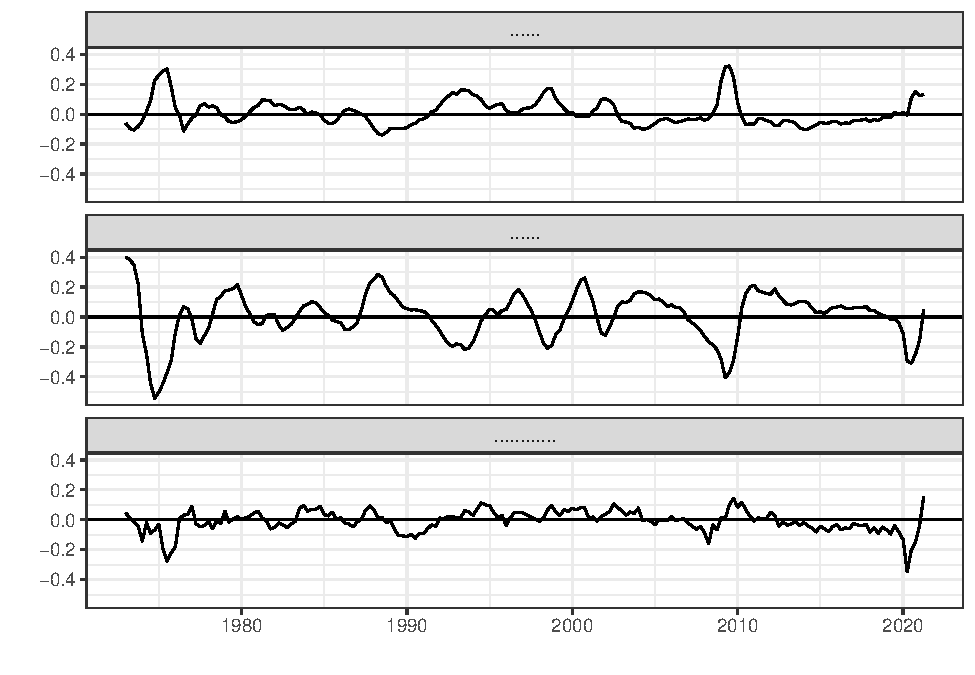
\includegraphics{test_files/figure-latex/unnamed-chunk-3-1.pdf}

\hypertarget{ux539aux751fux5206ux6790ux6642ux7cfbux5217ux6bd4ux8f03}{%
\chapter{厚生分析:時系列比較}\label{ux539aux751fux5206ux6790ux6642ux7cfbux5217ux6bd4ux8f03}}

\begin{itemize}
\tightlist
\item
  1963年から2020年までの年次データ、\citet{kawata2021first} の手法を用いて、求職者の厚生変化を記述する
\end{itemize}

\hypertarget{ux65b9ux6cd5-1}{%
\section{方法}\label{ux65b9ux6cd5-1}}

\begin{itemize}
\item
  同質な求職者・求人からなるモデルを用いて、識別のアイディアを紹介する。

  \begin{itemize}
  \tightlist
  \item
    \citet{kawata2021first} では異質性を導入・非定常であったとしても、同じ識別結果を得れることを示している
  \end{itemize}
\item
  標準的なDiamond-Mortencen-Pissarides型サーチモデル\citep{rogerson2005search}に準じて、以下の4条件式を仮定する
\end{itemize}

\begin{enumerate}
\def\labelenumi{\arabic{enumi}.}
\tightlist
\item
  失業者の価値関数は以下で定義される。
\end{enumerate}

\[rU=b+\underbrace{\Delta}_{サーチ活動の余剰}\]

ただし

\[\Delta = \underbrace{\frac{m}{u}}_{入職率}\times \underbrace{(W-U)}_{入職からの余剰}\]

\(m:\) 新規就職件数、\(u:\)求職者数、\(U:\)求職者の期待効用、\(W:\)就業者の期待効用、\(r,b:\) パラメータ

\begin{itemize}
\item
  総余剰をデータから識別することを目指す。

  \begin{itemize}
  \item
    同値はサーチ活動がもたらす期待余剰であり、入職率と入職がもたらす余剰\(W-U\)の積として定義されている。
  \item
    識別の障害となるのは、入職からの余剰をデータから直接観察できない点にある。以下では他の均衡条件を用いることで、この観察できない値の''変化''は復元できることを示している。
  \end{itemize}
\end{itemize}

\begin{enumerate}
\def\labelenumi{\arabic{enumi}.}
\setcounter{enumi}{1}
\tightlist
\item
  求人の価値関数は以下で定義される。
\end{enumerate}

\[rV=-k+\frac{m}{v}\times (J-V)\]

\(v:\) 求人数、\(m/v:\) 求人の充足率、\(J:\) 充足求人の期待利潤、\(V:\) 未充足求人の期待利潤、\(k:\) パラメータ

\begin{enumerate}
\def\labelenumi{\arabic{enumi}.}
\setcounter{enumi}{2}
\tightlist
\item
  自由参入条件は以下で定義される。
\end{enumerate}

\[V=0\]

\begin{itemize}
\tightlist
\item
  この条件は、未充足求人の期待利潤が0になるまで、新規求人が登録されることを仮定している。
\end{itemize}

\begin{enumerate}
\def\labelenumi{\arabic{enumi}.}
\setcounter{enumi}{3}
\tightlist
\item
  ナッシュ交渉
\end{enumerate}

\[(1-\beta)(W-U)=\beta(J-V)\]

\(\beta:\) パラメータ

\begin{itemize}
\tightlist
\item
  この条件は、マッチングによる余剰が、労働者と企業間でパラメータ\(\beta\)の割合で分配されることを仮定している。同パラメータをデータから推定することは困難であるが、以下の議論は、入職からの期待余剰\(\Delta\)の''変化''の識別は、\(\beta\)の識別を要求しないことを示している。
\end{itemize}

\hypertarget{ux8b58ux5225}{%
\subsection{識別}\label{ux8b58ux5225}}

\begin{itemize}
\tightlist
\item
  ナッシュ交渉より、入職からの余剰は以下のように書き換えられる。
\end{itemize}

\[\Delta = \underbrace{\frac{m}{u}}_{入職率}\times \underbrace{(W-U)}_{入職からの余剰}=\underbrace{\frac{m}{u}}_{入職率}\times \underbrace{\frac{\beta}{1-\beta}(J-V)}_{入職からの余剰}\]

\begin{itemize}
\tightlist
\item
  自由参入条件からさらに書き換えられる
\end{itemize}

\[\Delta = \underbrace{\frac{m}{u}}_{入職率}\times \underbrace{(W-U)}_{入職からの余剰}=\underbrace{\frac{m}{u}}_{入職率}\times \underbrace{\frac{\beta}{1-\beta}k\times\frac{v}{m}}_{入職からの余剰}\]

\begin{itemize}
\item
  同式からは、新規就職、求人、求職件数とパラメータの積により、新規就職からの余剰は書き下せる
  ことを示している。
\item
  未知のパラメータ(\(\beta\),\(k\))を含んでいるため\(\Delta\)そのものをデータから識別することはできないが、この対数差は識別可能である。
\item
  異なる状態(2019年 VS 2020年, ``With COVID-19'' VS ``Without COVID-19''等)におけるサーチ活動からの余剰を\(\Delta,\Delta'\)で記す。この対数差は
\end{itemize}

\[\log (\Delta) - \log(\Delta')=\underbrace{\log(\frac{m'}{u'})-\log(\frac{m}{u})}_{入職率の対数変化} + \underbrace{\log(\frac{v'}{m'})-\log(\frac{v}{m})}_{入職からの余剰の対数変化} = \log(\frac{v'}{u'})-\log(\frac{v}{u})\]

\begin{itemize}
\item
  同式職からの余剰は、求人倍率\(v/u\)の対数差により識別されることを示している。

  \begin{itemize}
  \tightlist
  \item
    さらにサーチ活動からの余剰は入職率、入職からの余剰の対数変化に分解でき、それぞれも新規就職・求人・求職件数のみで識別できることを示している。
  \end{itemize}
\end{itemize}

\hypertarget{ux6642ux7cfbux5217ux6bd4ux8f03ux3078ux306eux5fdcux7528}{%
\subsection{時系列比較への応用}\label{ux6642ux7cfbux5217ux6bd4ux8f03ux3078ux306eux5fdcux7528}}

\begin{itemize}
\item
  以下では前年同月と比べたサーチ活動からの余剰変化を推定している。

  \begin{itemize}
  \item
    例えば2020年4月については、\(\Delta=\) 2020年4月の余剰、\(\Delta'=\) 2019年4月の余剰を示す。
  \item
    同推定値は、前年に比べて求職者が置かれている状況が、どの程度改善ないし悪化しているのかを示す指標となる。
  \end{itemize}
\end{itemize}

\hypertarget{rux30b3ux30fcux30c9-1}{%
\section{Rコード}\label{rux30b3ux30fcux30c9-1}}

\begin{Shaded}
\begin{Highlighting}[]
\NormalTok{col.label }\OtherTok{\textless{}{-}} 
   \FunctionTok{c}\NormalTok{(}\StringTok{"year"}\NormalTok{,}
     \StringTok{"1"}\NormalTok{,}
     \StringTok{"2"}\NormalTok{,}
     \StringTok{"3"}\NormalTok{,}
     \StringTok{"4"}\NormalTok{,}
     \StringTok{"5"}\NormalTok{,}
     \StringTok{"6"}\NormalTok{,}
     \StringTok{"7"}\NormalTok{,}
     \StringTok{"8"}\NormalTok{,}
     \StringTok{"9"}\NormalTok{,}
     \StringTok{"10"}\NormalTok{,}
     \StringTok{"11"}\NormalTok{,}
     \StringTok{"12"}\NormalTok{,}
     \StringTok{"type"}\NormalTok{,}
     \StringTok{"group"}\NormalTok{)}

\NormalTok{select.raw }\OtherTok{\textless{}{-}} \DecValTok{14}\SpecialCharTok{:}\DecValTok{63}

\NormalTok{select.column }\OtherTok{\textless{}{-}} \FunctionTok{c}\NormalTok{(}\DecValTok{1}\NormalTok{,}\DecValTok{3}\SpecialCharTok{:}\DecValTok{14}\NormalTok{)}

\NormalTok{raw.vacancy.full }\OtherTok{\textless{}{-}}
  \FunctionTok{read\_excel}\NormalTok{(}\StringTok{"data/第6表.xlsx"}\NormalTok{,}
             \AttributeTok{sheet =} \StringTok{"第6表ー2(パート除く)"}\NormalTok{) }\SpecialCharTok{\%\textgreater{}\%}
\NormalTok{  .[select.raw,select.column] }\SpecialCharTok{|}\ErrorTok{\textgreater{}} 
  \FunctionTok{mutate}\NormalTok{(}\AttributeTok{type =} \StringTok{"求人"}\NormalTok{,}
         \AttributeTok{group =} \StringTok{"フルタイム"}\NormalTok{)}

\FunctionTok{colnames}\NormalTok{(raw.vacancy.full) }\OtherTok{\textless{}{-}}\NormalTok{ col.label}

\NormalTok{raw.seeker.full }\OtherTok{\textless{}{-}}
  \FunctionTok{read\_excel}\NormalTok{(}\StringTok{"data/第7表.xlsx"}\NormalTok{,}
             \AttributeTok{sheet =} \StringTok{"第7表ー2(パート除く)"}\NormalTok{) }\SpecialCharTok{\%\textgreater{}\%}
\NormalTok{  .[select.raw,select.column] }\SpecialCharTok{|}\ErrorTok{\textgreater{}} 
  \FunctionTok{mutate}\NormalTok{(}\AttributeTok{type =} \StringTok{"求職"}\NormalTok{,}
         \AttributeTok{group =} \StringTok{"フルタイム"}\NormalTok{)}

\FunctionTok{colnames}\NormalTok{(raw.seeker.full) }\OtherTok{\textless{}{-}}\NormalTok{ col.label}

\NormalTok{raw.hir.full }\OtherTok{\textless{}{-}}
  \FunctionTok{read\_excel}\NormalTok{(}\StringTok{"data/第8表.xlsx"}\NormalTok{,}
             \AttributeTok{sheet =} \StringTok{"第8表ー2(パート除く)"}\NormalTok{) }\SpecialCharTok{\%\textgreater{}\%}
\NormalTok{  .[select.raw,select.column] }\SpecialCharTok{|}\ErrorTok{\textgreater{}} 
  \FunctionTok{mutate}\NormalTok{(}\AttributeTok{type =} \StringTok{"新規就職"}\NormalTok{,}
         \AttributeTok{group =} \StringTok{"フルタイム"}\NormalTok{)}

\FunctionTok{colnames}\NormalTok{(raw.hir.full) }\OtherTok{\textless{}{-}}\NormalTok{ col.label}


\NormalTok{raw.vacancy.part }\OtherTok{\textless{}{-}}
  \FunctionTok{read\_excel}\NormalTok{(}\StringTok{"data/第6表.xlsx"}\NormalTok{,}
             \AttributeTok{sheet =} \StringTok{"第6表ー3(パート)"}\NormalTok{) }\SpecialCharTok{\%\textgreater{}\%}
\NormalTok{  .[select.raw,select.column] }\SpecialCharTok{|}\ErrorTok{\textgreater{}} 
  \FunctionTok{mutate}\NormalTok{(}\AttributeTok{type =} \StringTok{"求人"}\NormalTok{,}
         \AttributeTok{group =} \StringTok{"パートタイム"}\NormalTok{)}

\FunctionTok{colnames}\NormalTok{(raw.vacancy.part) }\OtherTok{\textless{}{-}}\NormalTok{ col.label}

\NormalTok{raw.seeker.part }\OtherTok{\textless{}{-}}
  \FunctionTok{read\_excel}\NormalTok{(}\StringTok{"data/第7表.xlsx"}\NormalTok{,}
             \AttributeTok{sheet =} \StringTok{"第7表ー3(パート)"}\NormalTok{) }\SpecialCharTok{\%\textgreater{}\%}
\NormalTok{  .[select.raw,select.column] }\SpecialCharTok{|}\ErrorTok{\textgreater{}} 
  \FunctionTok{mutate}\NormalTok{(}\AttributeTok{type =} \StringTok{"求職"}\NormalTok{,}
         \AttributeTok{group =} \StringTok{"パートタイム"}\NormalTok{)}

\FunctionTok{colnames}\NormalTok{(raw.seeker.part) }\OtherTok{\textless{}{-}}\NormalTok{ col.label}

\NormalTok{raw.hir.part }\OtherTok{\textless{}{-}}
  \FunctionTok{read\_excel}\NormalTok{(}\StringTok{"data/第8表.xlsx"}\NormalTok{,}
             \AttributeTok{sheet =} \StringTok{"第8表ー3(パート)"}\NormalTok{) }\SpecialCharTok{\%\textgreater{}\%}
\NormalTok{  .[select.raw,select.column] }\SpecialCharTok{|}\ErrorTok{\textgreater{}} 
  \FunctionTok{mutate}\NormalTok{(}\AttributeTok{type =} \StringTok{"新規就職"}\NormalTok{,}
         \AttributeTok{group =} \StringTok{"パートタイム"}\NormalTok{)}

\FunctionTok{colnames}\NormalTok{(raw.hir.part) }\OtherTok{\textless{}{-}}\NormalTok{ col.label}

\NormalTok{df }\OtherTok{\textless{}{-}}
  \FunctionTok{rbind}\NormalTok{(raw.hir.full,}
\NormalTok{        raw.hir.part,}
\NormalTok{        raw.vacancy.full,}
\NormalTok{        raw.vacancy.part,}
\NormalTok{        raw.seeker.full,}
\NormalTok{        raw.seeker.part}
\NormalTok{        ) }\SpecialCharTok{|}\ErrorTok{\textgreater{}} 
  \FunctionTok{pivot\_longer}\NormalTok{(}\AttributeTok{cols =} \DecValTok{2}\SpecialCharTok{:}\DecValTok{13}\NormalTok{,}
               \AttributeTok{names\_to =} \StringTok{"month"}\NormalTok{,}
               \AttributeTok{values\_to =} \StringTok{"n"}\NormalTok{) }\SpecialCharTok{|}\ErrorTok{\textgreater{}} 
  \FunctionTok{mutate}\NormalTok{(}\AttributeTok{n =}\NormalTok{ n }\SpecialCharTok{|}\ErrorTok{\textgreater{}} \FunctionTok{as.numeric}\NormalTok{(),}
         \AttributeTok{year =}\NormalTok{ year }\SpecialCharTok{|}\ErrorTok{\textgreater{}} \FunctionTok{str\_sub}\NormalTok{(}\DecValTok{1}\NormalTok{,}\DecValTok{4}\NormalTok{) }\SpecialCharTok{|}\ErrorTok{\textgreater{}} \FunctionTok{as.numeric}\NormalTok{(),}
         \AttributeTok{month =}\NormalTok{ month }\SpecialCharTok{|}\ErrorTok{\textgreater{}} \FunctionTok{as.numeric}\NormalTok{(),}
         \AttributeTok{quaterly =}\NormalTok{ month }\SpecialCharTok{|}\ErrorTok{\textgreater{}} \FunctionTok{cut}\NormalTok{(}\FunctionTok{c}\NormalTok{(}\DecValTok{0}\NormalTok{,}\DecValTok{3}\NormalTok{,}\DecValTok{6}\NormalTok{,}\DecValTok{9}\NormalTok{,}\DecValTok{12}\NormalTok{), }\AttributeTok{labels =} \FunctionTok{c}\NormalTok{(}\DecValTok{1}\NormalTok{,}\DecValTok{2}\NormalTok{,}\DecValTok{3}\NormalTok{,}\DecValTok{4}\NormalTok{)),}
         \AttributeTok{date =} \FunctionTok{yq}\NormalTok{(}\FunctionTok{str\_c}\NormalTok{(year,quaterly,}\AttributeTok{sep =} \StringTok{":Q"}\NormalTok{))}
\NormalTok{         ) }\SpecialCharTok{|}\ErrorTok{\textgreater{}} 
  \FunctionTok{group\_by}\NormalTok{(date,type) }\SpecialCharTok{|}\ErrorTok{\textgreater{}} 
  \FunctionTok{mutate}\NormalTok{(}\AttributeTok{n =}\NormalTok{ n }\SpecialCharTok{|}\ErrorTok{\textgreater{}} \FunctionTok{sum}\NormalTok{()) }\SpecialCharTok{|}\ErrorTok{\textgreater{}} 
  \FunctionTok{ungroup}\NormalTok{() }\SpecialCharTok{|}\ErrorTok{\textgreater{}} 
  \FunctionTok{distinct}\NormalTok{(year,quaterly,date,type,n) }\SpecialCharTok{|}\ErrorTok{\textgreater{}} 
  \FunctionTok{spread}\NormalTok{(}\AttributeTok{key =}\NormalTok{ type, }\AttributeTok{value =}\NormalTok{ n) }\SpecialCharTok{|}\ErrorTok{\textgreater{}} 
  \FunctionTok{group\_by}\NormalTok{(quaterly) }\SpecialCharTok{|}\ErrorTok{\textgreater{}} 
  \FunctionTok{mutate}\NormalTok{(入職率 }\OtherTok{=} \FunctionTok{log}\NormalTok{(新規就職}\SpecialCharTok{/}\NormalTok{求職) }\SpecialCharTok{{-}} \FunctionTok{log}\NormalTok{(}\FunctionTok{lag}\NormalTok{(新規就職}\SpecialCharTok{/}\NormalTok{求職)),}
\NormalTok{         マッチングの余剰 }\OtherTok{=} \FunctionTok{log}\NormalTok{(}\FunctionTok{lag}\NormalTok{(新規就職}\SpecialCharTok{/}\NormalTok{求人)) }\SpecialCharTok{{-}} \FunctionTok{log}\NormalTok{(新規就職}\SpecialCharTok{/}\NormalTok{求人),}
\NormalTok{           総余剰 }\OtherTok{=} \FunctionTok{log}\NormalTok{(求人}\SpecialCharTok{/}\NormalTok{求職) }\SpecialCharTok{{-}} \FunctionTok{log}\NormalTok{(}\FunctionTok{lag}\NormalTok{(求人}\SpecialCharTok{/}\NormalTok{求職))}
\NormalTok{           ) }\SpecialCharTok{|}\ErrorTok{\textgreater{}} 
  \FunctionTok{ungroup}\NormalTok{() }\SpecialCharTok{|}\ErrorTok{\textgreater{}} 
  \FunctionTok{select}\NormalTok{(}\SpecialCharTok{{-}}\NormalTok{求職,}
         \SpecialCharTok{{-}}\NormalTok{求人,}
         \SpecialCharTok{{-}}\NormalTok{新規就職) }\SpecialCharTok{|}\ErrorTok{\textgreater{}} 
  \FunctionTok{pivot\_longer}\NormalTok{(}\AttributeTok{cols =} \FunctionTok{c}\NormalTok{(}\DecValTok{4}\SpecialCharTok{:}\DecValTok{6}\NormalTok{),}
               \AttributeTok{names\_to =} \StringTok{"type"}\NormalTok{,}
               \AttributeTok{values\_to =} \StringTok{"N"}\NormalTok{) }\SpecialCharTok{|}\ErrorTok{\textgreater{}} 
  \FunctionTok{na.omit}\NormalTok{()}

\NormalTok{fig }\OtherTok{\textless{}{-}}
\NormalTok{  df }\SpecialCharTok{|}\ErrorTok{\textgreater{}} 
  \FunctionTok{ggplot}\NormalTok{(}\FunctionTok{aes}\NormalTok{(}\AttributeTok{x =}\NormalTok{ date,}
             \AttributeTok{y =}\NormalTok{ N)}
\NormalTok{         ) }\SpecialCharTok{+}
  \FunctionTok{geom\_line}\NormalTok{() }\SpecialCharTok{+}
  \FunctionTok{geom\_hline}\NormalTok{(}\AttributeTok{yintercept =} \DecValTok{0}\NormalTok{) }\SpecialCharTok{+}
  \FunctionTok{facet\_wrap}\NormalTok{(}\SpecialCharTok{\textasciitilde{}}\FunctionTok{factor}\NormalTok{(type,}
                     \AttributeTok{levels =} \FunctionTok{c}\NormalTok{(}\StringTok{"マッチングの余剰"}\NormalTok{,}
                                \StringTok{"入職率"}\NormalTok{,}
                                \StringTok{"総余剰"}\NormalTok{)),}
             \AttributeTok{ncol =} \DecValTok{1}\NormalTok{) }\SpecialCharTok{+}
  \FunctionTok{ylab}\NormalTok{(}\StringTok{""}\NormalTok{) }\SpecialCharTok{+}
  \FunctionTok{xlab}\NormalTok{(}\StringTok{""}\NormalTok{) }\SpecialCharTok{+}
  \FunctionTok{theme\_bw}\NormalTok{()}
\end{Highlighting}
\end{Shaded}

\hypertarget{ux7d50ux679c-1}{%
\section{結果}\label{ux7d50ux679c-1}}

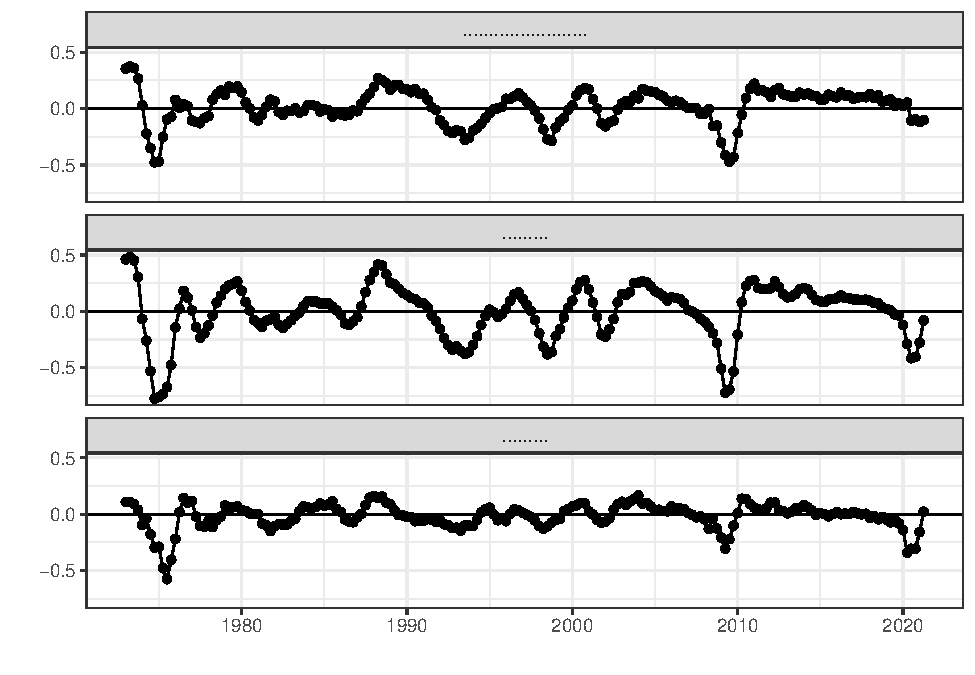
\includegraphics{test_files/figure-latex/unnamed-chunk-5-1.pdf}

\hypertarget{session-information}{%
\chapter{Session information}\label{session-information}}

\begin{Shaded}
\begin{Highlighting}[]
\FunctionTok{sessionInfo}\NormalTok{()}
\end{Highlighting}
\end{Shaded}

\begin{verbatim}
## R version 4.1.0 (2021-05-18)
## Platform: x86_64-w64-mingw32/x64 (64-bit)
## Running under: Windows 10 x64 (build 19042)
## 
## Matrix products: default
## 
## locale:
## [1] LC_COLLATE=Japanese_Japan.932  LC_CTYPE=Japanese_Japan.932   
## [3] LC_MONETARY=Japanese_Japan.932 LC_NUMERIC=C                  
## [5] LC_TIME=Japanese_Japan.932    
## 
## attached base packages:
## [1] stats     graphics  grDevices utils     datasets  methods   base     
## 
## other attached packages:
##  [1] knitr_1.33       lubridate_1.7.10 readxl_1.3.1     forcats_0.5.1   
##  [5] stringr_1.4.0    dplyr_1.0.7      purrr_0.3.4      readr_1.4.0     
##  [9] tidyr_1.1.3      tibble_3.1.2     ggplot2_3.3.5    tidyverse_1.3.1 
## 
## loaded via a namespace (and not attached):
##  [1] tidyselect_1.1.1  xfun_0.24         haven_2.4.1       colorspace_2.0-1 
##  [5] vctrs_0.3.8       generics_0.1.0    htmltools_0.5.1.1 yaml_2.2.1       
##  [9] utf8_1.2.1        rlang_0.4.11      pillar_1.6.1      glue_1.4.2       
## [13] withr_2.4.2       DBI_1.1.1         dbplyr_2.1.1      modelr_0.1.8     
## [17] lifecycle_1.0.0   munsell_0.5.0     gtable_0.3.0      cellranger_1.1.0 
## [21] rvest_1.0.0       evaluate_0.14     labeling_0.4.2    fansi_0.5.0      
## [25] highr_0.9         broom_0.7.8       Rcpp_1.0.6        backports_1.2.1  
## [29] scales_1.1.1      jsonlite_1.7.2    farver_2.1.0      fs_1.5.0         
## [33] hms_1.1.0         digest_0.6.27     stringi_1.6.1     bookdown_0.22    
## [37] grid_4.1.0        cli_2.5.0         tools_4.1.0       magrittr_2.0.1   
## [41] pacman_0.5.1      crayon_1.4.1      pkgconfig_2.0.3   ellipsis_0.3.2   
## [45] xml2_1.3.2        reprex_2.0.0      assertthat_0.2.1  rmarkdown_2.9    
## [49] httr_1.4.2        rstudioapi_0.13   R6_2.5.0          compiler_4.1.0
\end{verbatim}

  \bibliography{book.bib,packages.bib}

\end{document}
